\chapter{The Lord's Prayer (Part 1: Father)}
\vspace{0.6cm}
\begin{center}
\nopagebreak
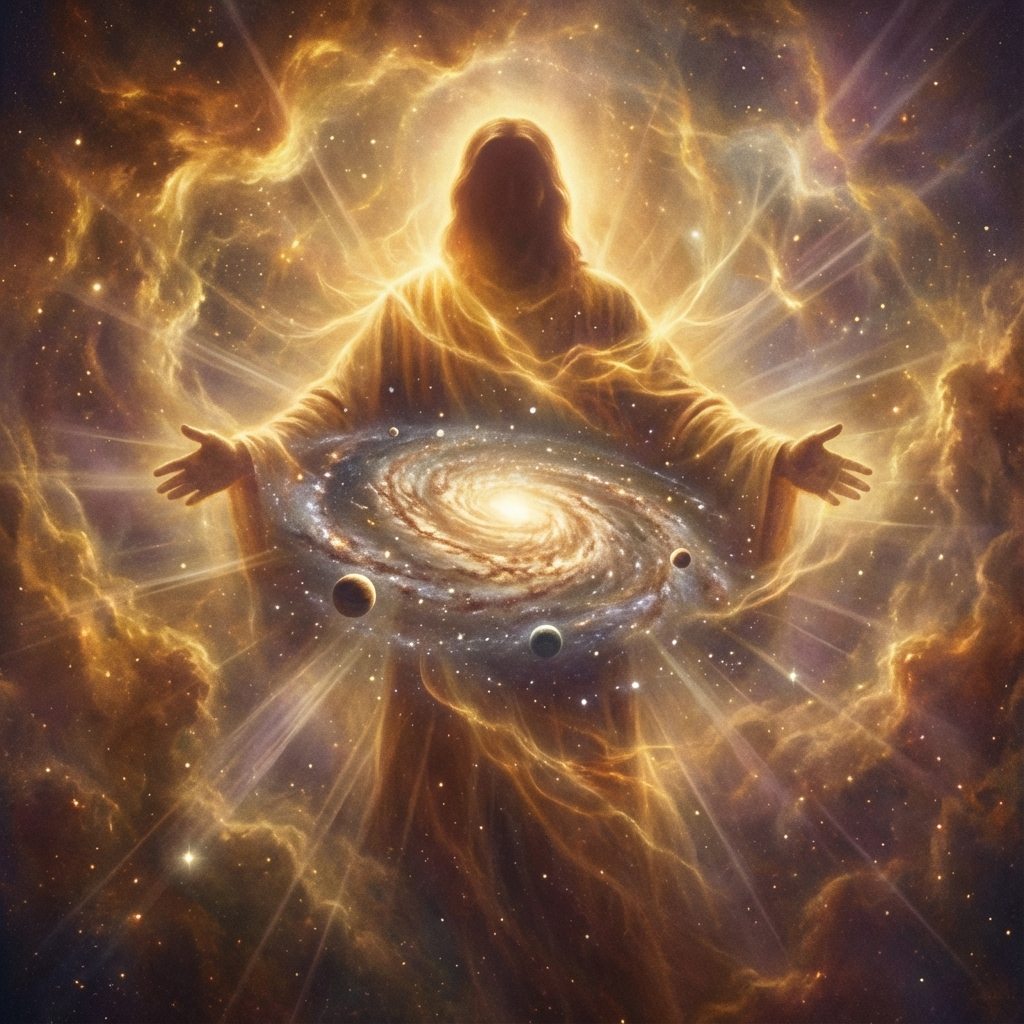
\includegraphics[width=0.75\textwidth,cfbox=gray!60 0.6pt 4pt]{cosmic_father.png}\\
\vspace{4pt}
{\small\itshape Abwoon: the cosmic Source of all creation.}
\end{center}

\vspace{0.6cm}
We returned to Madrid, but this time we went to Retiro. We sat near the Crystal Palace.
—Let's talk about your father —Jesus said suddenly.


I tensed up. My relationship with my father had not always been easy.
—Why?


—Because the prayer starts with ``Our Father''. And many people get stuck there. If your earthly father was harsh, or absent, or critical, you project that image onto God. You believe that God is a gentleman with a beard who watches you to punish you if you make a mistake.


He picked up a stone from the ground and threw it into the pond. The ripples expanded.
—The word ``Father'' in Aramaic, \textit{Abwoon}, has a much broader meaning. It is the Source, the Origin, the Breath of Life. It's not a gentleman. It's an Energy. It's the original vibration from which we all come.


—So, he's not a judge?


—Of course not! —he exclaimed—. Does the sun judge the flowers? Does it say to them ``you do bloom, I give you light; you do not, you stay in the dark''? The sun shines for all. God is unconditional Love. If you close yourself in a cave, it's not the sun's fault that you're in the dark. It's your choice.


—And why ``Our''?


—Because it's not ``Mine''. It's not the private property of any religion, nor of any person. It belongs to everyone. To the Christian, the Buddhist, the atheist, the tree and the dog. We all come from the same Source. Recognizing that is the first step to vibrate high: Unity. If you see yourself as separate from others, you lower your vibration. If you see yourself as united, you go up.